%Use pdfLaTeX to compile

\documentclass[12pt,a4paper]{report}
\usepackage[pdftex]{graphicx}
\usepackage{titletoc} 
\usepackage{fancyhdr}   
\usepackage[a4paper,pdftex]{geometry}	
\usepackage[english]{babel}
\usepackage{xcolor} 
\usepackage{enumerate}
\usepackage{fix-cm} 
\usepackage[notlof]{tocbibind}
\usepackage{amsmath}
\usepackage{listings}
\usepackage{hyperref}
\usepackage{caption}
\usepackage{float}
\usepackage{graphicx}
\usepackage{subcaption}
\usepackage{upquote}
\usepackage{listings}
\definecolor{dkgreen}{rgb}{0,.6,0}
\definecolor{dkblue}{rgb}{0,0,.6}
\definecolor{dkyellow}{cmyk}{0,0,.8,.3}
 \captionsetup[figure]{font=small}
\bibliographystyle{ieeetr}  
\usepackage[toc,page]{appendix}

\lstset{
	language        = php,
	basicstyle      = \small\ttfamily,
	keywordstyle    = \color{dkblue},
	stringstyle     = \color{red},
	identifierstyle = \color{dkgreen},
	commentstyle    = \color{gray},
	emph            =[1]{php},
	emphstyle       =[1]\color{black},
	emph            =[2]{if,and,or,else},
	emphstyle       =[2]\color{dkyellow}}
\lstdefinelanguage{javascript}{
	morekeywords={break, case, catch, continue, debugger, default, delete,         do, else, false, finally, for, function, if, in, instanceof, new, null, return, switch, this, throw, true, try, typeof, var, void, while, with},
	morecomment=[s]{/*}{*/},
	morecomment=[l]//,
	morestring=[b]",
	morestring=[b]'
}
\lstdefinelanguage{css}{
	keywords={accelerator,azimuth,background,background-attachment,
		background-color,background-image,background-position,
		background-position-x,background-position-y,background-repeat,
		behavior,border,border-bottom,border-bottom-color,
		border-bottom-style,border-bottom-width,border-collapse,
		border-color,border-left,border-left-color,border-left-style,
		border-left-width,border-right,border-right-color,
		border-right-style,border-right-width,border-spacing,
		border-style,border-top,border-top-color,border-top-style,
		border-top-width,border-width,bottom,caption-side,clear,
		clip,color,content,counter-increment,counter-reset,cue,
		cue-after,cue-before,cursor,direction,display,elevation,
		empty-cells,filter,float,font,font-family,font-size,
		font-size-adjust,font-stretch,font-style,font-variant,
		font-weight,height,ime-mode,include-source,
		layer-background-color,layer-background-image,layout-flow,
		layout-grid,layout-grid-char,layout-grid-char-spacing,
		layout-grid-line,layout-grid-mode,layout-grid-type,left,
		letter-spacing,line-break,line-height,list-style,
		list-style-image,list-style-position,list-style-type,margin,
		margin-bottom,margin-left,margin-right,margin-top,
		marker-offset,marks,max-height,max-width,min-height,
		min-width,-moz-binding,-moz-border-radius,
		-moz-border-radius-topleft,-moz-border-radius-topright,
		-moz-border-radius-bottomright,-moz-border-radius-bottomleft,
		-moz-border-top-colors,-moz-border-right-colors,
		-moz-border-bottom-colors,-moz-border-left-colors,-moz-opacity,
		-moz-outline,-moz-outline-color,-moz-outline-style,
		-moz-outline-width,-moz-user-focus,-moz-user-input,
		-moz-user-modify,-moz-user-select,orphans,outline,
		outline-color,outline-style,outline-width,overflow,
		overflow-X,overflow-Y,padding,padding-bottom,padding-left,
		padding-right,padding-top,page,page-break-after,
		page-break-before,page-break-inside,pause,pause-after,
		pause-before,pitch,pitch-range,play-during,position,quotes,
		-replace,richness,right,ruby-align,ruby-overhang,
		ruby-position,-set-link-source,size,speak,speak-header,
		speak-numeral,speak-punctuation,speech-rate,stress,
		scrollbar-arrow-color,scrollbar-base-color,
		scrollbar-dark-shadow-color,scrollbar-face-color,
		scrollbar-highlight-color,scrollbar-shadow-color,
		scrollbar-3d-light-color,scrollbar-track-color,table-layout,
		text-align,text-align-last,text-decoration,text-indent,
		text-justify,text-overflow,text-shadow,text-transform,
		text-autospace,text-kashida-space,text-underline-position,top,
		unicode-bidi,-use-link-source,vertical-align,visibility,
		voice-family,volume,white-space,widows,width,word-break,
		word-spacing,word-wrap,writing-mode,z-index,zoom},  
	sensitive=true,
	morecomment=[l]{//},
	morecomment=[s]{/*}{*/},
	morestring=[b]',
	morestring=[b]",
	alsoletter={:},
	alsodigit={-}
}
\begin{document}
\begin{titlepage}
\begin{center}

\includegraphics[scale=1.5]{figures/CoverSheet}\\
\bf{ \small{DEPARTMENT OF ELECTRICAL AND ELECTRONIC ENGINEERING} }
\end{center}

\vspace{18mm}
 \begin{center}
 \begin{Large}
 {EEE212 Group Project}\\ 
 \vspace{2.0cm}
 \bf{Smart House: Remote Light Control}
 \end{Large}
 \end{center} 
\vspace{2.0cm}

  \begin{center}
  \begin{large}
     \begin{tabular}{r@{ }l} 
     	
     	\bf{Group Number :} &  Group 7\\
     \end{tabular}
 \vspace{2.0cm}
	\begin{table}[H]
		\centering
		\begin{tabular}{c l c }
			\bf{Student Name and ID}& Sahand Sabour&1614650\\
			&Jiamin Wang&1613827\\
			&Tingyu Lin&1611905\\
			&Mengqing Zhao&1613288\\
			&Kai-Yu Lu&1614649\\
			
		\end{tabular}
	\end{table}
\vspace{1.0cm}
\begin{tabular}{r@{ }l} 
	
	\bf{Supervisor and Assessor : }&  Tiew On Ting\\
\end{tabular}
	
  \end{large}
  \end{center}
\clearpage
\end{titlepage}

\abstract{
	Begun in the early 2000s, major companies have been emphasizing on a concept that could revolutionize the way we live our daily lives; the Smart House. The Internet of Things (IoT) is the foundation of this concept as it allows us to establish a network between home appliances. 
	\vspace{0.2cm}
	
	\noindent This project aims to build a small prototype of the Smart House concept; where a user can use our WeChat mini-program to control and monitor the lights in the house model as well as its front door. In this report, we would explain the methodology that we used for developing this model and provide test results of the final product. Moreover, we will discuss the problems and limitations that our team faced during the development of this project and would provide plans for the future of this project likewise. 
	\vspace{0.2cm}
	
	\noindent In conclusion, our team is able to successfully build a properly functioning prototype of the Smart House concept with short response time and low rate of failure. We sincerely believe that working on this project allowed us to investigate several important concepts such as Internet of Things and hardware programming. We also believe that it helped us improve our team working and communication skills.
	 
}

\tableofcontents


\quad 
\setcounter{page}{1}
\chapter{Introduction}
\section{Background}
As technology grows, the need for connectivity rises. In the modern world, being able to remotely control one's electric and electronic possessions has become one of the main objectives of great companies (e.g., Apple, Google, and Amazon) due to its considerable impact in daily lives and its growing market. The rise of Internet of Things (IoT) has been the main cause for this growth. Internet of Things can be defined as a group of devices (things) that are interconnected within a network\cite{IOT}. IoT provides a much larger platform for sharing information compared to the Internet and the concept of Smart house was invented as a result of this phenomenon\cite{SmartHouse}. 
 
\section{Objective}
This project aims to demonstrate a small model of the Smart House. A user can use our WeChat mini program to control power supply to the house's lights and monitor the current status of its door. Our team used an ESP8266 Wi-Fi module to establish the network within the house. Moreover, we deployed an online server to conduct the required communications between the module and the mini-program. This report includes thorough explanation of both the hardware and software of this project as well as the corresponding working principles, testing results, and discussions for each case. 

\section{Literature Review}
The Smart House concept applies technologies regarding embedded systems and network communications to construct a digital residence system. It covers an energy-saving design and integration of telecommunications to build a functional network of home appliances which are constantly in communication. This network of devices allows remote access to monitor and manage home appliances, which would be more time-efficient and convenient from a house owner’s perspective \cite{lolz}. 

\vspace{0.2cm}
\noindent However, this concept has never been able to reach the consumer acceptance and adoption levels that many other technologies have achieved. This is not only due to its deployment price but is also due to the privacy and security issues that a Smart House might have as well as lack of consumers' trust \cite{haha}. Moreover, the amount of research regarding user satisfaction towards Smart House is insignificant. Hence, there have been several barriers that have declined its rate of development and improvement. Therefore, raising customer awareness, acceptance, and trust would be a strong foundation for future development of the Smart House \cite{yaya}.


\chapter{Methodology} 
This section of the report demonstrates the design, development, and integration process of the Smart House project. Internet of Things (IOT), WeChat mini-program and web server development as well as wireless transmission methods comprise the subjects that are implemented in the development process. Moreover, the house model's circuitry consists of an ESP8266 WiFi module, a digital magnetic sensor, and three LED lights. 
\begin{figure}[H]
	\centering
	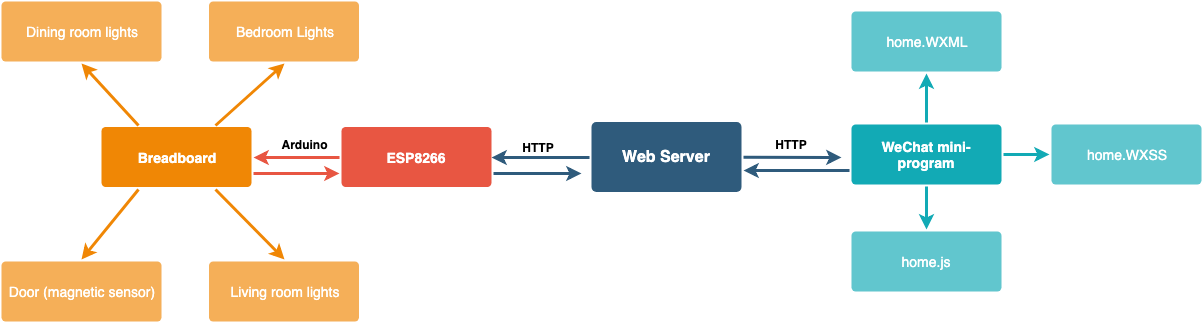
\includegraphics[height=6cm,width=16cm]{figures/system.PNG}
	\caption{Smart House System Architecture}
\end{figure}

\noindent The overall architecture of the system is shown in the above figure and its methodology can be divided into four main parts: House model design, Arduino design, mini-program design, and server design; we will demonstrate and thoroughly explain the mentioned methods in the following sections respectively. 

\vspace{10cm}
\section{House model design}
Our team built a small-scale model of the smart house system using cardboard and colored stickers. As the first step, we cut open a carton and removed one of its sides as it was regarded as the display side. This side would be used to display the whole inside of the model to the outside viewers. Consequently, our team connected a pink piece of cardboard to the top side of the carton to make the peaked roof and covered the whole inner sides of the model with colored stickers. Accordingly, we assembled a basic space frame with these sides and reinforced it with scotch tape. 

\vspace{0.1cm}


\noindent The model’s length, width and height are 29.1cm, 13.5cm, and 26.0cm respectively. As decided, the model would have two floors. The first floor would be the living room with a red LED with height of 14.0cm while the second floor would consist of the bedroom and the dining room with height of 12.0cm. In order to divide the model into two floors, we horizontally glued a piece of cardboard to the walls. Moreover, we used the clapboard to divide the two rooms on the second floor. Therefore, the room on the left would be the bedroom with a yellow LED and the other room would be the dining room with a green LED. 



\vspace{0.1cm}
\noindent As for the door of the house model, we designed a single door on the right side of the model with its height, width, and upper-threshold being 11.9cm, 6.8cm, and 0.8 centimeter-high respectively. Subsequently, we installed a magnetic sensor on the upper-side of the door-frame while adding a magnet to the top of the door. With this approach, the magnet and the sensor will be fairly close when the door is closed and far away when the door is open. Conclusively, we placed the Arduino board on the backside of the model. The following figure displays the resulting house model.


\vspace{0.2cm}
\begin{figure}[H]
	\centering
	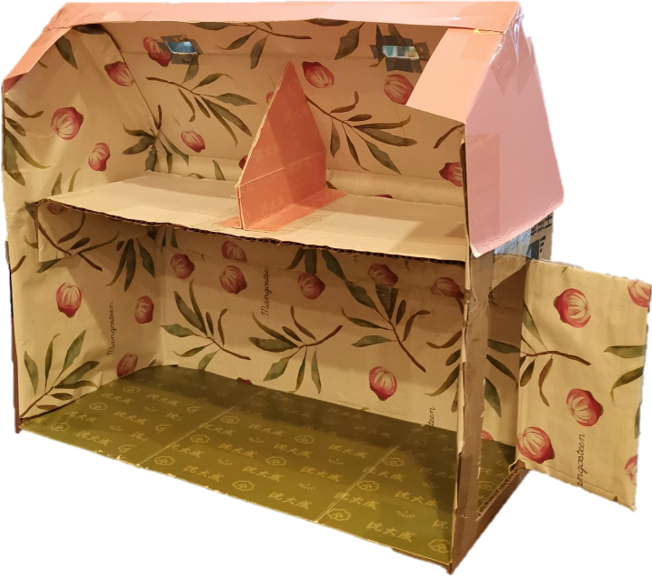
\includegraphics[height=6cm,width=8cm]{figures/house.png}
	\caption{House model}
\end{figure}

\section{Arduino design}
Arduino is an open-source application which relies on both hardware and software for designing diverse prototypes. The combination of boards and programming is flexible enough for beginners to generate an expected design \cite{arduino}. The Arduino board allows reading of the inputs and generates corresponding outputs based on users’ instructions. Arduino UNO is a basic hardware device with 14 digital input/output pins and 6 analog inputs. It can be driven by an external power supply or USB connection \cite{arduino2}. The core part of designing this project is implementing the required functionalities via the Arduino Software (IDE) \cite{arduino}.
\subsection{Circuit Design}
To implement the Internet of Things (IoT) and create a network between the house model's LED lights and door, our team initially decided to implement the ESP8266 Wi-Fi module. However, the connection between ESP8266 module and a basic Arduino UNO board was slightly complicated to establish; thus, we used a NodeMCU board, which has the fundamental functions of both the Arduino UNO and the Wi-Fi module ESP8266 \cite{nodemcu}.
\begin{figure}[H]
	\centering
	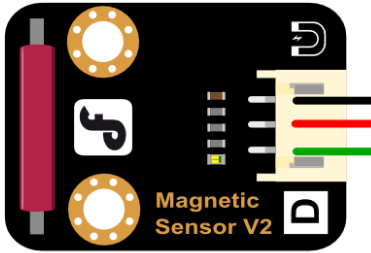
\includegraphics[width=5cm]{figures/sensor.png}
	\caption{The digital magnetic sensor}
\end{figure}
\noindent 
For each LED, we connected its longer leg (the anode) to one of the digital pins while connecting the other leg (the cathode) to the ground (GND). As for the digital magnetic sensor, the green line was connected to the digital pin, the red line was connected to the 3.3V supply pin while the black line was connected to the ground (check Figure 2.3). The magnetic sensor is quite sensitive and can easily be influenced by other parts of the circuit. Therefore, to avoid this problem, we added a large value resistor ($15k\Omega$) between the digital pin and the GND pin. The following figure displays the assembled circuit (Figure 2.4).

\begin{figure}[H]
	\centering
	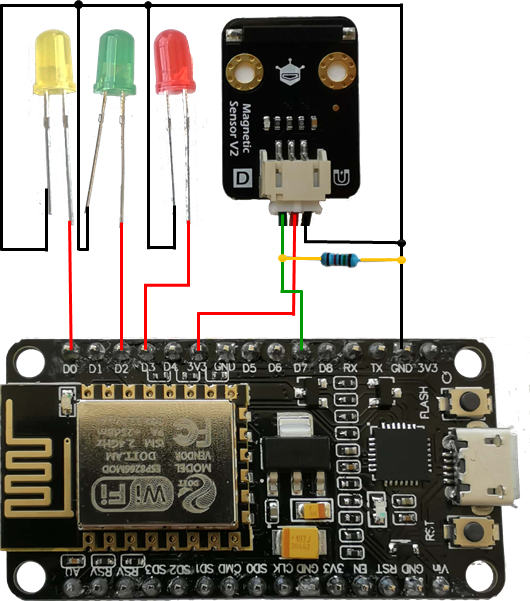
\includegraphics[height=6cm, width=8cm]{figures/circuit.png}
	\caption{The Arduino circuitry}
\end{figure}




\subsection{Programming}
In the Arduino Software (IDE), the digital pins can be used as either input or output. The pinMode() function is used to declare a pin variable as an input or output \cite{arduino2}. In this project, we defined pins for LEDs as outputs and the pin for the magnetic sensor as input. Regarding the connections between inputs and outputs, the digitalWrite() function would assign a value to an output pin while the digitalRead() function reads a value from an input pin \cite{arduino2}.

\vspace{0.1cm}

\noindent As for the Wi-Fi implementation, we used the following two libraries: 


\vspace{0.2cm}
\noindent \textbf{$<$ESP8266WiFi.h$>$} For Connecting to a Wi-Fi network such as a router. 

\vspace{0.2cm}

\noindent \textbf{$<$ESP8266HTTPClient.h$>$} For sending HTTP requests and returning the results. The program would process the response with pin information to link the new updates with the LED lights and the sensor on the board. 

\vspace{0.2cm}
\noindent As we will mention in section 2.4.2, HTTP requests are essential to the functionality of this project. Our Arduino program would send two types of requests:


\noindent \textbf{GET requests} obtain the current status of each light in the house, whether on or off. Based on our team's decision, the program would send a get request to the server every second to ensure the that the lights in the house are updated accordingly. 

\vspace{0.1cm}

\noindent \textbf{SET requests} update the current status of the door in the database (open/closed). The program does not send these requests to the server automatically and would only send them when the status of the digital magnetic sensor changes. 
\vspace{0.1cm}

\noindent check appendices for the code for Arduino setup codes.

\begin{figure}[H]
	\centering
	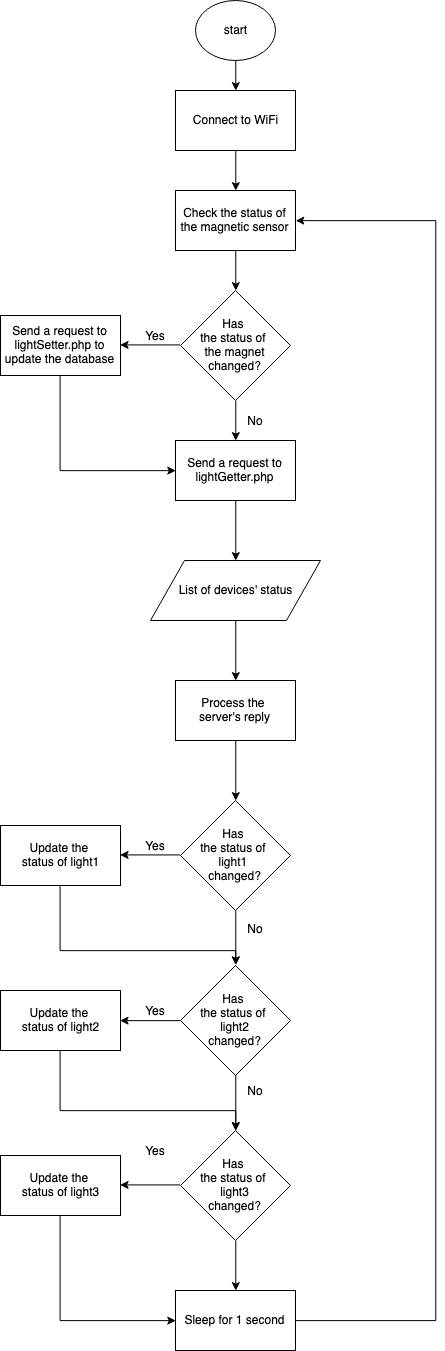
\includegraphics[scale= 0.43]{figures/arduinoFlow.png}
	\caption{Flowchart for the Arduino program}
\end{figure}

\section{Mini-program design}
WeChat mini-programs have become fairly popular during the past couple of years. They are sub-applications that can run within the WeChat app's environment. These mini-apps lack many functionalities that a normal app would provide, such as being able to send notifications and run in an independent environment; however, they also provide functionalities that are not available when developing an IOS or Android app. By using Tencent's development kits, our team was able to write a program that would run on any device that has WeChat preinstalled regardless of the device's operating system. This is the main reason why our team chose this platform for developing the app.
\subsection{User Interface}
The user Interface is what the users interact with when they use the mini-app; this is the visual side of the program. The UI provides the user with ability to interact with the server and update the database without any complexity. We used WXML and WXSS, which are the WeChat mini-app equivalents of HTML and CSS, to display the data from the server while providing an easy-to-use, stylish environment. The following figure the results from final stage of the WeChat mini-app's UI development:
\begin{figure}[H]
	\begin{subfigure}{.3\textwidth}
		\centering
		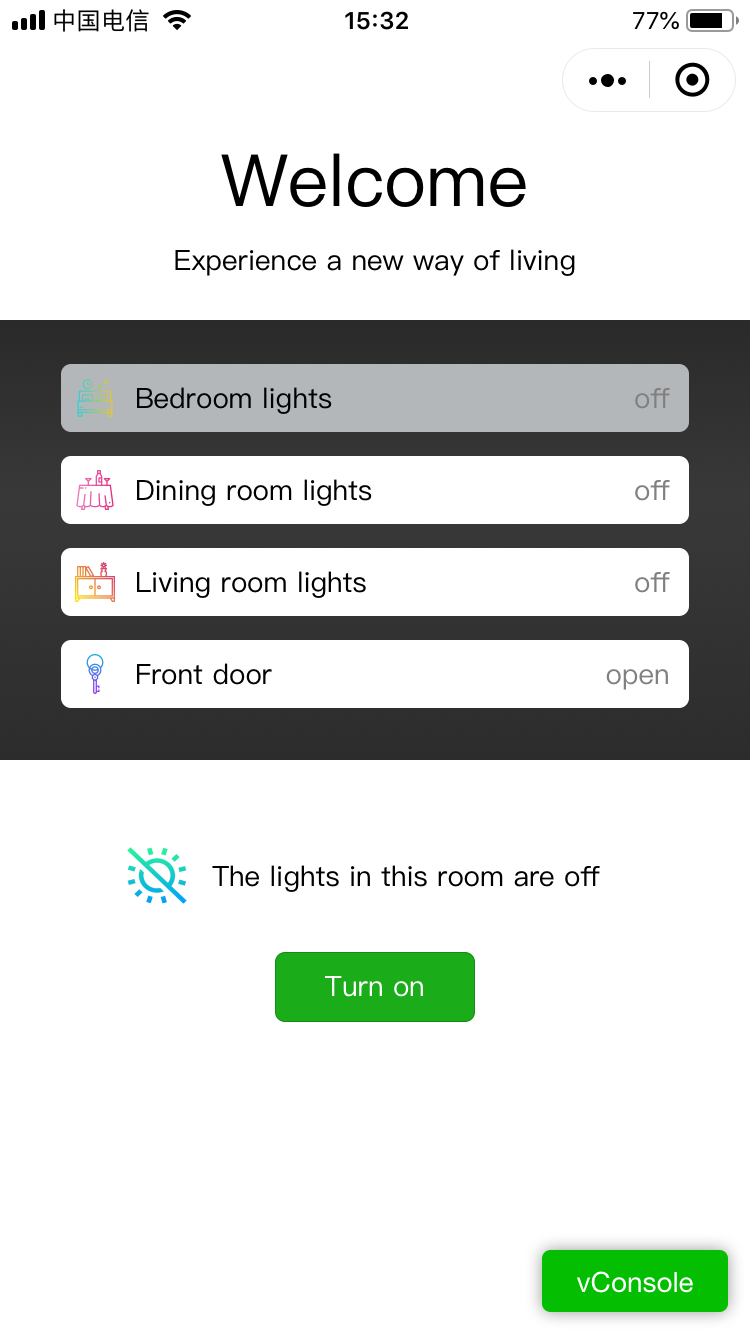
\includegraphics[width=.8\linewidth]{figures/1.png}
		\caption{Light on}
	\end{subfigure}
	\begin{subfigure}{.3\textwidth}
		\centering
		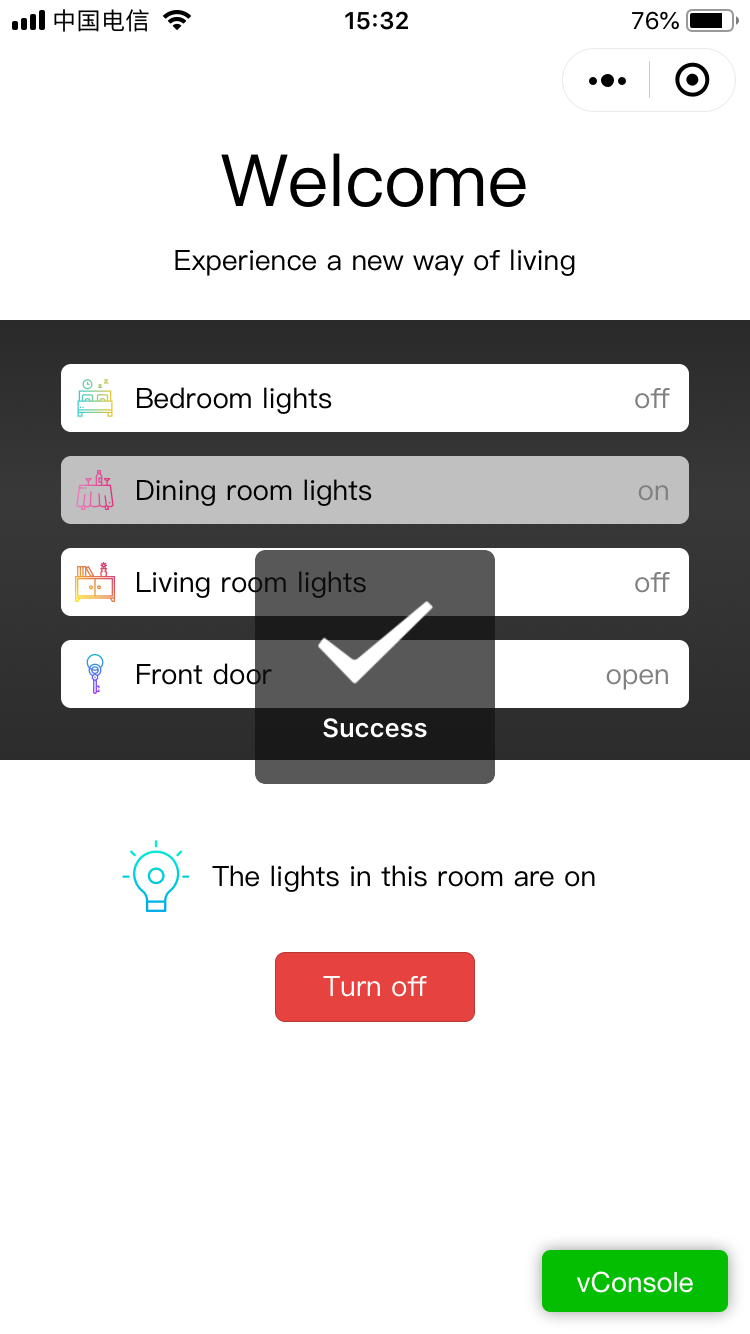
\includegraphics[width=.8\linewidth]{figures/2.png}
		\caption{Turning light off}
	\end{subfigure}
\begin{subfigure}{.3\textwidth}
	\centering
	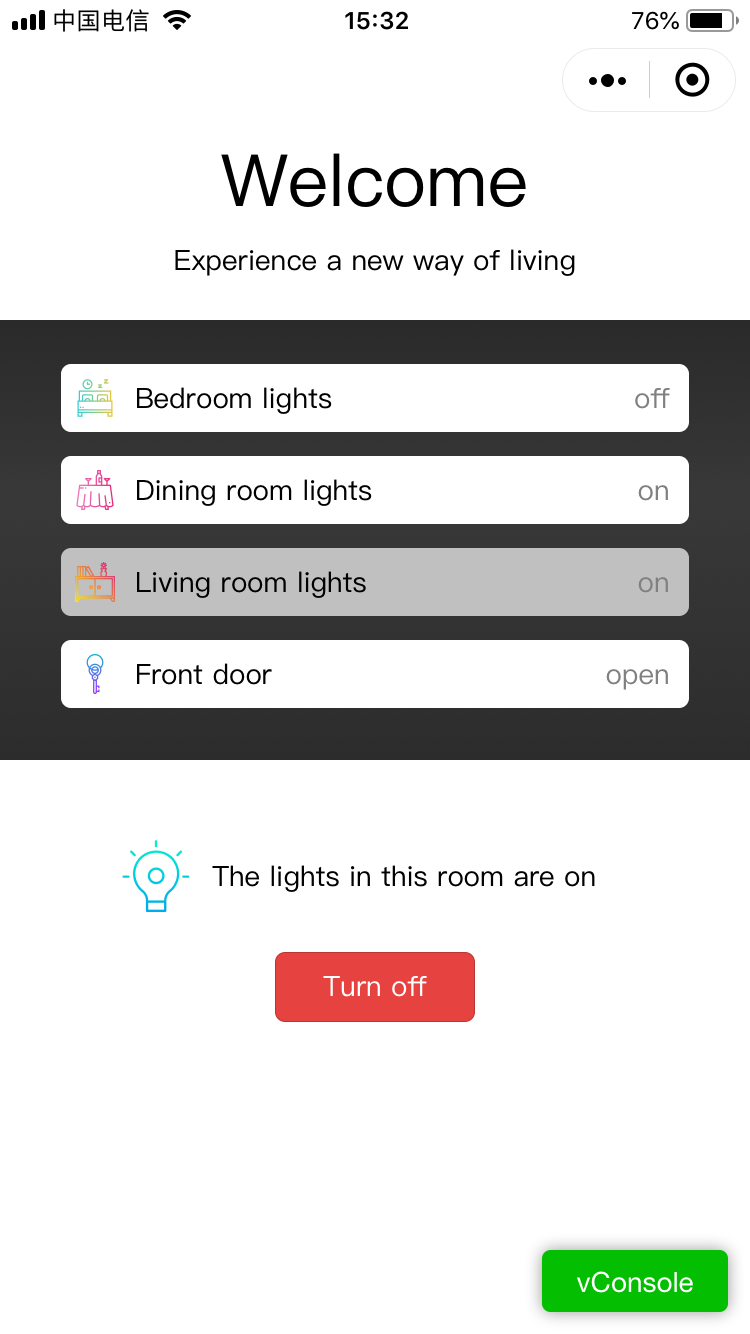
\includegraphics[width=.8\linewidth]{figures/3.png}
	\caption{Light off}
\end{subfigure}
\end{figure}

\begin{figure}[H]
	\begin{subfigure}{.5\textwidth}
		\centering
		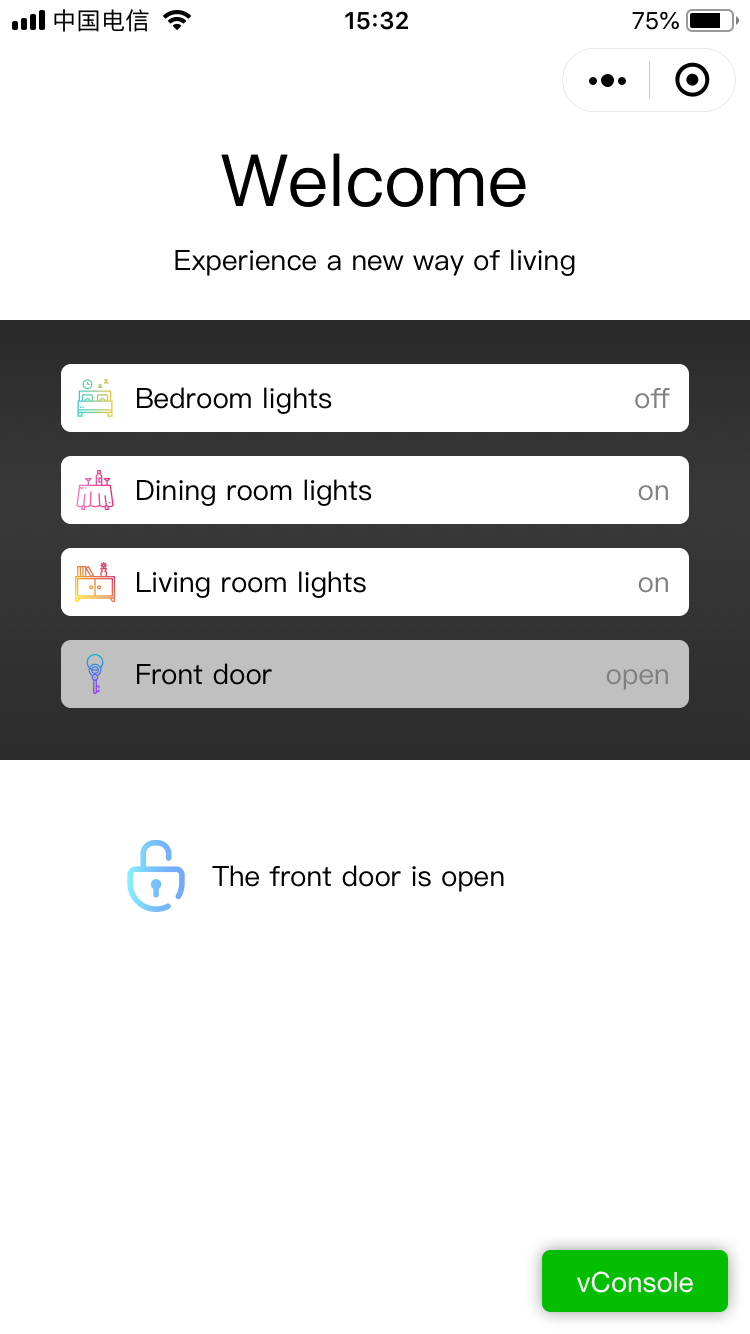
\includegraphics[height=6cm, width=.5\linewidth]{figures/4.png}
		\caption{Door open}
	\end{subfigure}
	\begin{subfigure}{.5\textwidth}
		\centering
		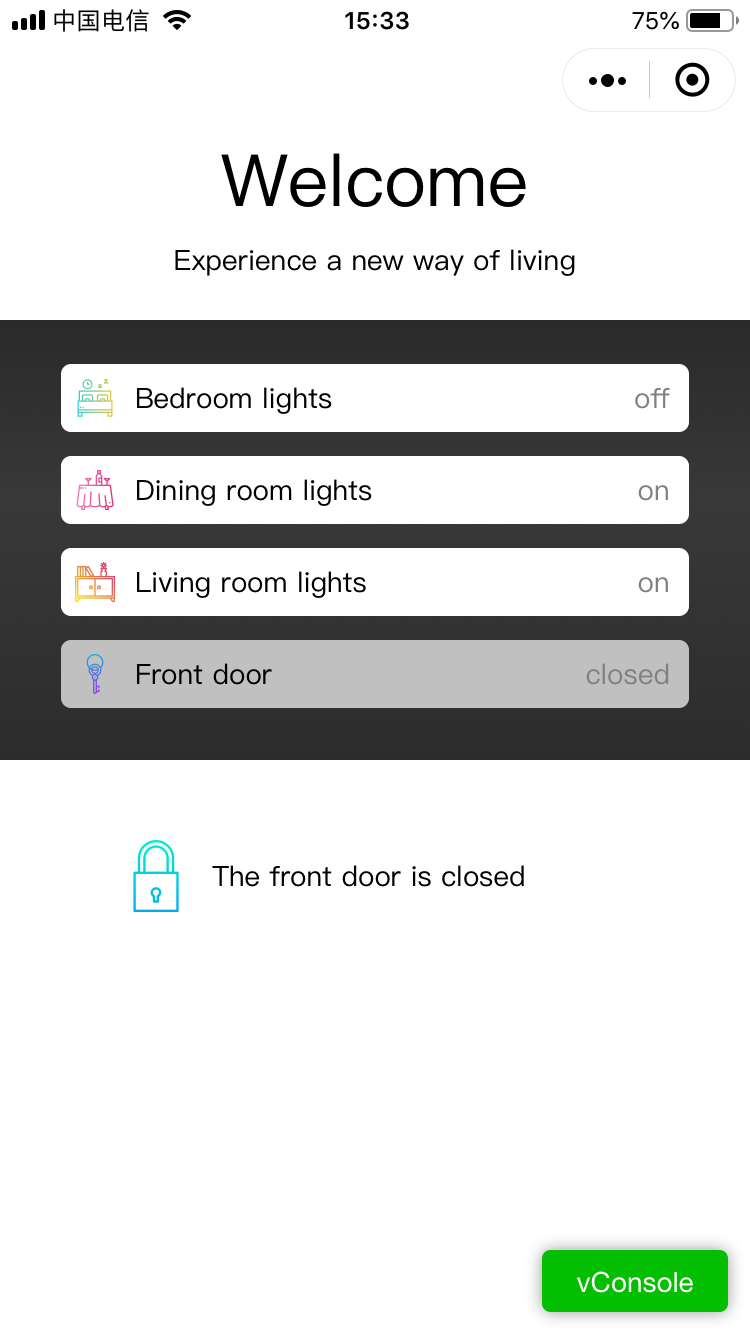
\includegraphics[height=6cm, width=.5\linewidth]{figures/5.png}
		\caption{Door closed}
	\end{subfigure}
\end{figure}

\begin{figure}[H]
	\begin{subfigure}{.5\textwidth}
		\centering
		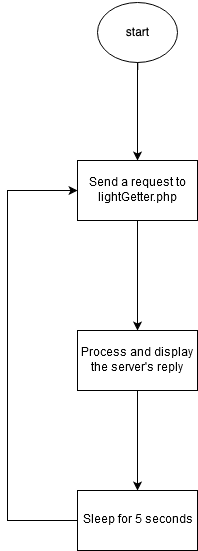
\includegraphics[height= 10cm, width=.5\linewidth]{figures/miniFlow1.png}
		\caption{Flowchart for receiving data}
	\end{subfigure}
	\begin{subfigure}{.5\textwidth}
		\centering
		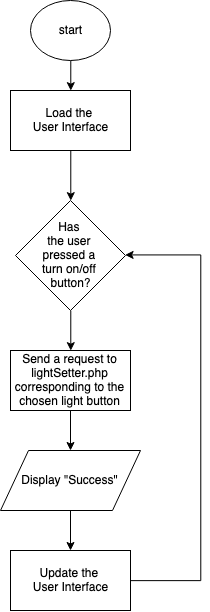
\includegraphics[height= 10cm,width=.5\linewidth]{figures/miniFlow2.png}
		\caption{Flowchart for sending data}
	\end{subfigure}
\end{figure}



\subsection{HTTP Requests}
In order to communicate with the server, either to receive data or update the database, the mini-app has to send HTTP requests to the server. We used JavaScript as the programming language for sending these requests, receiving replies from the server, processing the obtained data. 

\noindent This program consists of two types of requests, namely get and set. 
\vspace{0.15cm}

\noindent \textbf{Get requests} obtain the current status of each light in the house, whether on or off, as well as the current status of the house's door, whether open or closed. As decided by our team, a get request is sent to the server every five seconds to ensure the reliability of the displayed data.

\vspace{0.15cm}

\noindent \textbf{Set requests} update the current status of each light in the database (turn on/off). These requests are not sent to the server automatically and would only be sent the user taps the button for turning on/off a specified light.
\vspace{0.3cm}

\noindent check appendices for the code for WeChat mini-program codes.

\section {Server design}
The server is the most fundamental part of this project; it acts as a communication bridge between the circuitry in the house model and the mini-app. A properly functioning server is expected to store the specified data in its database and respond to received requests with proper responses. The hosting plan for this project was purchased from \url{www.000webhost.com}, which included \url{eeearduino.000webhostapp.com} as the domain, a preconfigured MySQL database, and support for PHP as a back-end programming language. 


\subsection{Database}
Our team used the database to store the current status of each light as well as the state of the house door respectively. We used MySQL as the programming language to design the database on the mentioned server. Hence, we created a row of four columns to store the data. The columns are as follows: 
\vspace{0.15cm}

\noindent \textbf{light1} corresponding to the bedroom lights, 
\vspace{0.15cm}

\noindent\textbf{light2} corresponding to the Dining room lights,
 \vspace{0.15cm}
 
\noindent\textbf{light3} corresponding to the lights in the living room, and 

\vspace{0.15cm}
\noindent\textbf{doorlock} corresponding to the state of the house door.

\vspace{0.3cm}

\noindent check appendices for the SQL codes of creating and initializing the table.

\subsection{Web Server}
We used PHP as the programming language for developing the web server. Consequently, The following two PHP files were created and added to the server:
\vspace{0.15cm}

\noindent \textbf{lightGetter.php} This file would return the value of each row from the database, which would correspond to the status of the lights and the house door respectively. This information is useful for updating the status table in both the ESP8266 module and the mini-app.
\vspace{0.15cm}

\noindent \textbf{lightSetter.php} This file would get two attributes from the client and update the database accordingly. The mentioned attributes correspond respectively to which device's status should be updated and what the new status of this device is. 
\vspace{0.3cm}

\noindent check appendices for the codes of the above PHP files.

\begin{figure}[H]
	\begin{subfigure}{.5\textwidth}
		\centering
		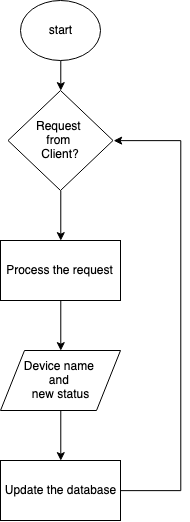
\includegraphics[width=.5\linewidth]{figures/lightSetter.png}
		\caption{Flowchart for lightSetter.php}
	\end{subfigure}
	\begin{subfigure}{.5\textwidth}
		\centering
		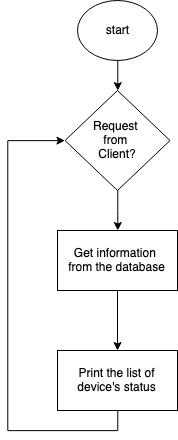
\includegraphics[height= 10cm, width=.5\linewidth]{figures/lightGetter.png}
		\caption{Flowchart for lightGetter.php}
	\end{subfigure}
\end{figure}

\chapter{Result and Discussion}
The project builds a prototype of smart home technology, and achieves the remote information transmission through implementation of IoT. Specifically, a user can use mobile devices to control the lights and check the status of door via WeChat mini-program. The following tests were designed to evaluate the efficiency and accuracy of the project.
\section{Testing results}
The magnetic force and transmission time were analyzed respectively; using the control variate method. Moreover, the constant supply voltage is 5.1 V / 2.1 A. By controlling the number of magnets, the magnetic induction ranges with the transmission time of door and lights status changes were measured (See Tables 3.1 and 3.2). 

\begin{enumerate}
	\item \textbf{Door}
	
	Initially, the distance between the magnets and the magnetic sensor were measured. For one magnet, the magnetic induction range was from 2mm to 8mm; the magnetic induction range of two magnets wass expanded from 10mm to 22mm. Consequently, we carried out ten sets of tests for one magnet and two magnets respectively.
	\begin{figure}[H]
		\centering
		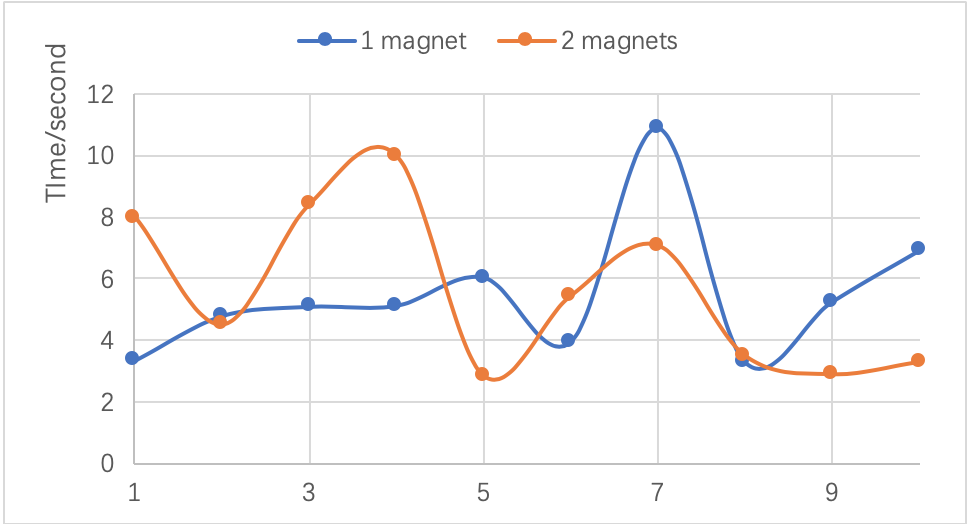
\includegraphics[height=6cm,width=12cm]{figures/door.PNG}
		\caption{Transmission time for change of door status}
	\end{figure}
	\begin{table}[H]
		\centering
		\begin{tabular}{|c|c|c|}
			\hline
			&1 magnet (s)&2 magnets (s)\\ 
			&(2mm-8mm)&(10mm-22mm)\\ \hline
			1&3.357&8.006\\ \hline
			2&	4.8	&4.519
\\ \hline
			3&	5.107&	8.406
\\ \hline
			4&	5.138&	9.992
\\ \hline
			5&	6.055&	2.868
\\ \hline
			6&	3.963&	5.444
\\ \hline
			7&	10.894&	7.088
\\ \hline
			8&	3.319&	3.523
\\ \hline
			9&	5.275&	2.914
\\ \hline
			10&	6.92&	3.308
\\ \hline
			Average&	5.481&	5.6068
\\ \hline

		\end{tabular}
		\label{Door statement transmission time}
		\caption{Door statement transmission time}
	\end{table}
According to the above table, the average transmission time of the two status were 5.481s and 5.6068s. Without considering changes in network speed, the transmission time of the door statement was not involved in the magnetic force. Due to the size of the model, we only used one magnet to obtain more accurate sensing results.

\vspace{10cm}
\item \textbf{Light}

\begin{figure}[H]
	\centering
	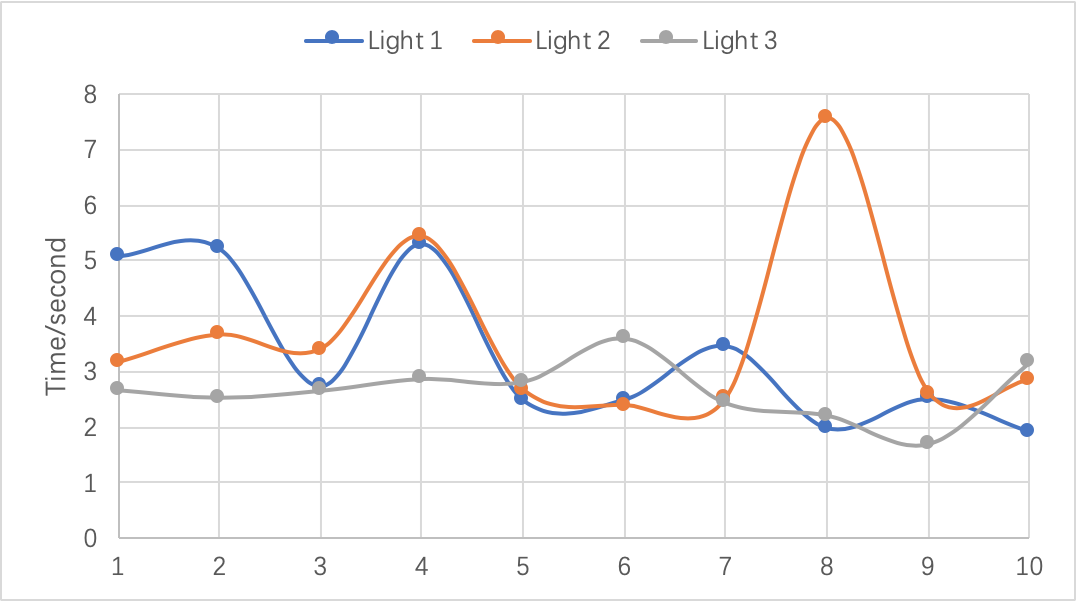
\includegraphics[height=6cm,width=12cm]{figures/light.PNG}
	\caption{Transmission time for change of light status}
\end{figure}

The following table contains the transmission time of the LED lights:
\begin{table}[H]
	\centering
	\begin{tabular}{|c|c|c|c|}
		\hline
		&L1(s)&L2(s)&L3(s)\\ \hline
		1&	5.082&	3.165&	2.672
\\ \hline
		2&	5.221&	3.664&	2.538
\\ \hline
		3&	2.739&	3.407&	2.661
\\ \hline
		4&	5.306&	5.442&	2.872
\\ \hline
		5&	2.491&	2.672&	2.822
\\ \hline
		6&	2.501&	2.392&	3.595
\\ \hline
		7&	3.466&	2.524&	2.441
\\ \hline
		8&	1.986&	7.578&	2.218
\\ \hline
		9&	2.514&	2.618&	1.71
\\ \hline
		10&	1.917&	2.846&	3.167
\\ \hline
		Average&	3.3223&	3.6308&	2.6696
\\ \hline
	\end{tabular}
	\label{Light transmission time}
	\caption{Light transmission time}
\end{table}

From Table 3.2, the average transmission time for the lights is about 3.208s. With an stable network connection, the success rate would reach approximately 100\%.
\end{enumerate}

\vspace{10cm}
\section{Discussion}

Based on the results of the previous chapter, we can observe that the response time for the transmission is within an acceptable range and the success rates are approximately 100\%. This chapter intends to discuss the results and analyze the relative merits of this project. 

\vspace{0.2cm}

\noindent From Tables 3.1 and 3.2, we can conclude that the transmission time, response time, and the rate of success are acceptable. This conclusion is due to the average time for completing the operations being within 5 seconds. However, we can observe that some groups of data are unstable. For instance, in terms of the dining room lights, one of the experimental transmission times is 7.5s, which is approximately twice the average time whose value is 3.2076s. Additionally, the data for the lock state of transmission time is also includes instances that take twice the average time of transmission. Therefore, we should improve the stability of the project in future. 

\vspace{0.2cm}

\noindent As we discussed previously, the I/O pin is sensitive to electrical noise. Hence, it will cause random fluctuations in I/O between LOW and HIGH; which would cause a phenomenon known as the floating pin. This is shown in Figure 3.3. 

\begin{figure}[H]
	\centering
	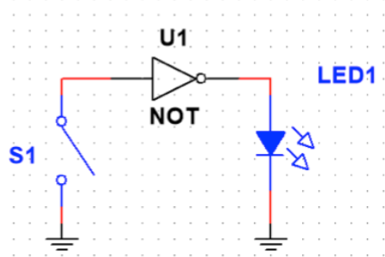
\includegraphics[scale= 1]{figures/badFP.png}
	\caption{Bad design causing floating pin}
\end{figure}

\vspace{0.2cm}

\noindent In order to avoid the floating pin, we inserted a pull-up 15 k$\Omega$ resistor between IO and GND pins (check Figure 3.4). During the data testing process, we discovered that the mistakes caused by electrical noise had been removed so this method successfully address the raised problem. 

\begin{figure}[H]
	\centering
	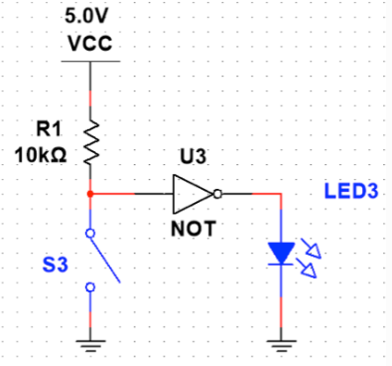
\includegraphics[scale= 1]{figures/goodFP.png}
	\caption{The design for avoiding “Floating pin” }
\end{figure}

\vspace{0.2cm}
\noindent Traditionally, the time for switching the lights can be limited to less than a second; although the average time for switching the lights remotely is 3.2 seconds with occasional errors. Hence, the design for networking should be improved in future. 


\chapter{Improvement}
As we discussed in the previous chapter, we expect several improvements in the stability and the design of the network. Therefore, this section intends to discuss several practical and efficient methods to improve the stability and address the concerns regarding the transmission time. 
\vspace{0.2cm}

\noindent 4G is the current method of Internet transmission, whose transmission rate is approximately 100Mbps. Various digital applications implement this technology; however, many news sources have recently highlited the technology of 5G, whose transmission rate would reach 10Gbps (100 times faster than 4G). Moreover, the delay for 4G is 30-50 milliseconds, however, the delay for 5G is theoretically 1 milliseconds, which means the implementation of 5G in our project can enhance the transmission time and decrease the failure rate. Therefore, 5G is a technical-edge and promising method that could improve our project in the future. As our current server is located in the USA, development of a server in the local country could also be beneficial. 


\vspace{0.2cm}

\noindent Regarding the security issues and privacy concerns of this prototype, we plan to add owner authorization, user verification, and data encryption to our WeChat mini-program to address this issue. Consequently, we would provide a unique digital key for each user which would resemble the physical house key in terms of usage.




\chapter{Conclusion}
In conclusion, by utilizing Arduino programming and circuitry, WeChat development tools, and web servers, our team was able to successfully build a properly functioning prototype of the Smart House, where the user can control and monitor the lights in the house as well as its front door.

\vspace{0.2cm}
\noindent Our team believes that working on this project allowed us to investigate several important subjects such as the Internet of Things (IoT) and Hardware programming. It also enabled us to improve our team working and communication skills.  We sincerely hope that we can persist on improving this prototype and produce a complete product in the future. 


\bibliographystyle{IEEEtran}
\bibliography{ref}

\begin{appendices}
\begin{verbatim}
The code for the Arduino:

#include <ESP8266WiFi.h>
#include <ESP8266HTTPClient.h>

const char* ssid =""; //your ssid
const char* password= ""; //your password

char* light1= "off";
char* light2= "off";
char* light3= "off";

int ledPin1 = 16; //D0 // GPIO2 of ESP8266
int ledPin2 = 4;  //D2
int ledPin3 = 0;  //D3
int inputPinhey = 13; // choose the input pin
int oldval=0;
int changeState=LOW;

const char* host="eeearduino.000webhostapp.com";

int arrayIndex= 0;
String ourResponse;

void setup() {
Serial.begin(115200);
delay(10);

pinMode(ledPin1, OUTPUT);
pinMode(ledPin2, OUTPUT);
pinMode(ledPin3, OUTPUT);
pinMode(inputPinhey, INPUT);
digitalWrite(ledPin1, LOW);
digitalWrite(ledPin2, LOW);
digitalWrite(ledPin3, LOW);

Serial.println();
Serial.println();
Serial.println("Connecting to ");
Serial.println(ssid);

WiFi.begin(ssid, password);

while(WiFi.status() != WL_CONNECTED){
delay(500);
Serial.print(".");
}
Serial.println();
Serial.println("Wifi connected");
Serial.println("IP:");
Serial.println(WiFi.localIP());
}

void loop() {

char* door="open";

int val = digitalRead(inputPinhey);

//Setter
Serial.println("Value: ");
Serial.println(String(val));
if (val==HIGH){ //Door closed
door="closed";
Serial.println("Door: ");
Serial.println(door);
}
else{
door="open";
Serial.println("Door: ");
Serial.println(door);
}

HTTPClient http1;  //Declare an object of class HTTPClient

http1.begin("http://eeearduino.000webhostapp.com/lightSetter.php?lightNum=doorlock&status="+String(door));  //Specify request destination
int httpCode1 = http1.GET();                                                                  //Send the request

if (httpCode1 > 0) { //Check the returning code

String payload1 = http1.getString();   //Get the request response payload
Serial.println(payload1);                     //Print the response payload

}

http1.end();   //Close connection


//GETTER
HTTPClient http;  //Declare an object of class HTTPClient

//Specify request destination
http.begin("http://eeearduino.000webhostapp.com/lightGetter.php");  

//Send the request
int httpCode = http.GET();                                                                  

if (httpCode > 0) { //Check the returning code

String payload = http.getString();   //Get the request response payload
Serial.println(payload);                     //Print the response payload
if (payload.substring(0,2) =="on"){
light1="on";

//on on 
if (payload.substring(3, 5) =="on"){
light2="on";
//on on on
if (payload.substring(6,8) =="on"){
light3="on";
}
else{
light3="off";
}
}

//on off
else{
light2="off";
//on off on
if (payload.substring(7,9) =="on"){
light3="on";
}
else{
light3="off";
}
}
}

//Light 1 is off
else{

light1="off";
//off on
if (payload.substring(4,6) =="on"){
light2="on";
//off on on
if (payload.substring(7,9) =="on"){
light3="on";
}
else{
light3="off";
}
}

// off off
else{
light2="off";
//off off on
if (payload.substring(8,10) =="on"){
light3="on";
}
else{
light3="off";
}
}

}

Serial.println("light 1 ==>");
Serial.println(light1);
Serial.println("light 2 ==>");
Serial.println(light2);
Serial.println("light 3 ==>");
Serial.println(light3);
Serial.println("Closing connection...");

//Changing status of light 1
if(light1=="on"){
digitalWrite(ledPin1, HIGH);
}
else{
digitalWrite(ledPin1, LOW);
}

//Changing status of light 2
if(light2=="on"){
digitalWrite(ledPin2, HIGH);
}
else{
digitalWrite(ledPin2, LOW);
}

//Changing status of light 3
if(light3=="on"){
digitalWrite(ledPin3, HIGH);
}
else{
digitalWrite(ledPin3, LOW);
}
}

http.end();   //Close connection

delay(1000); 

}
\end{verbatim}

\vspace{4cm}
\begin{verbatim}
The code for home.wxml:
\end{verbatim}
\vspace{-0.5cm}
\begin{lstlisting}[language={html}]
<view id="pageTitle" class="ripple fadeInDown">Welcome</view>
<view id="pageSubtitle" class="ripple fadeInDown">
Experience a new way of living
</view>

<view id="content" style="opacity:{{showContent?'1':'0'}}">
<view class="iconLabel" bindtouchstart='changeLight' 
data-lightNum='1'  
style="background:{{selectedLight=='1'?'#B4B7BA':''}};">
<image class="iconImage" src="../../Images/bed.png"></image>
<view class="iconName">Bedroom lights</view>
<view class="iconStatus">{{lightStatus[0]}}</view>
</view>
<view class="iconLabel" bindtouchstart='changeLight' 
data-lightNum='2' 
style="background:{{selectedLight=='2'?'silver':''}};">
<image class="iconImage" src="../../Images/dinner.png"></image>
<view class="iconName">Dining room lights</view>
<view class="iconStatus">{{lightStatus[1]}}</view>
</view>
<view class="iconLabel" bindtouchstart='changeLight' 
data-lightNum='3' 
style="background:{{selectedLight=='3'?'silver':''}};">
<image class="iconImage" src="../../Images/room.png"></image>
<view class="iconName">Living room lights</view>
<view class="iconStatus">{{lightStatus[2]}}</view>
</view>
<view class="iconLabel" bindtouchstart='changeLight' 
data-lightNum='4' 
style="background:{{selectedLight=='4'?'silver':''}};">
<image class="iconImage" src="../../Images/key.png"></image>
<view class="iconName">Front door</view>
<view class="iconStatus">{{lightStatus[3]}}</view>
</view>
</view>

<view class="button_container" 
style="opacity: {{selectedLight!=null?'1':'0'}}">

<block wx-if="{{selectedLight!=null}}">
<view class="imageMessage">
<block wx-if="{{selectedLight!=4 &&selectedLight!=null}}">
<image class="lightPic" 
src="{{lightStatus[selectedLight-1]=='on'?'../../Images/lightOn.png':
'../../Images/lightOff.png'}}">
</image>
<view class="lightMessage">
The lights in this room are{{lightStatus[selectedLight-1]}}
</view>
</block>
<block wx-if="{{selectedLight==4}}">
<image class="lightPic" 
src="{{lightStatus[selectedLight-1]=='closed'?
'../../Images/lock.png':'../../Images/unlock.png'}}">
</image>
<view class="lightMessage">
The front door is {{lightStatus[selectedLight-1]}}</view>
</block>
</view>
<button class="button" bindtap="changeStatus"
type="{{lightStatus[selectedLight-1]=='on'?'warn':'primary'}}" 
disabled="{{disabled}}" 
style="display:{{selectedLight==4?'none':''}}">
{{lightStatus[selectedLight-1]=='on'?
'Turn off':'Turn on'}}</button>
</block>

</view>
\end{lstlisting}

\begin{verbatim}
The code for home.wxss:
\end{verbatim}
\vspace{-0.5cm}
\begin{lstlisting}[language={css}]
@import "../../CSS_files/ripples.wxss";

#pageTitle{
text-align: center;
font-size: 36px;
margin-bottom: 4px;
}

#pageSubtitle{
text-align: center;
font-size: 14px;
}

#content{
margin-top: 20px;
transition: 0.6s;
background: 
-webkit-linear-gradient(top, #323232 0%, #3F3F3F 40%, #1C1C1C 150%), 
-webkit-linear-gradient(bottom, rgba(255, 255, 255, 0.4) 0%, 
rgba(0, 0, 0, 0.25) 200%);
background: 
linear-gradient(to bottom, #323232 0%, #3F3F3F 40%, #1C1C1C 150%),
linear-gradient(to top, rgba(255, 255, 255, 0.4) 0%, 
rgba(0, 0, 0, 0.25) 200%);
background-blend-mode: multiply;
padding: 10px 0;
height: 200px;
}

.iconLabel{
width: 80%;
margin: 12px auto;
padding: 7px;
display: flex;
flex-direction: row;
background: white;
border-radius: 5px;
}

.iconImage{
height: 20px;
width: 20px;
display: block;
position: relative;
margin-right: 10px;
}

.iconName{
margin-top: 3px;
font-size: 14px;
line-height: 14px;
}

.iconStatus{
color: grey;
margin-top: 3px;
position: fixed;
font-size: 14px;
line-height: 14px;
right: 40px;
}

.lightContainer{
width: 100%;
display: flex;
flex-direction: row;
margin: 36px 0;
}

.lightBox{
display: inline-block;
width: 80px;
height: 80px;
border: 1px solid black;
margin-left: 32px;
border-radius: 50%;
transition: 0.3s;
}

.lightBox-text{
margin: auto;
width: 80px;
height: 16px;
text-align: center;
line-height: 16px;
font-size: 16px;
margin-top: 32px;
}

.button_container{
transition: 0.3s;
margin-top: 30px;
}

.button{
width: 100px;
font-size: 14px;
margin: auto;
transition: 0.3s;
}

.imageMessage{
display: flex;
flex-direction: row;
margin:10px auto;
padding: 10px;
transition: 0.3s;
}

.lightPic{
height: 36px;
width: 36px;
margin-left: 50px;
margin-right: 10px;
}

.lightMessage{
margin-top: 11px;
font-size: 14px;
line-height: 14px;
}
\end{lstlisting}

\begin{verbatim}
The code for home.js:
\end{verbatim}
\vspace{-0.5cm}
\begin{lstlisting}[language={javascript}]
Page({
data: {
opening: true,
showContent: false, 
disabled: false,
updating: false,
selectedLight: null,
lightStatus: ['off', 'off', 'off', 'closed'], 
disabled: false
},

changeStatus(){
var lightStatus= this.data.lightStatus
var selectedLight= this.data.selectedLight
if (lightStatus[selectedLight - 1] == "on"){
lightStatus[selectedLight - 1] = "off"
}
else{
lightStatus[selectedLight - 1] = "on"
}
this.setData({
lightStatus: lightStatus
})
console.log(this.data.lightStatus)
this.setLightData()
}
,
changeLight(e){
let lightNum = e.currentTarget.dataset.lightnum
if (lightNum== this.data.selectedLight){
lightNum=null;
}
this.setData({
selectedLight: parseInt(lightNum)
})
}
,
getLightData(){
var that = this;
if (this.data.opening){
wx.showLoading({
title: 'Downloading',
})
}

if(!this.data.updating){
wx.request({
url: 'https://eeearduino.000webhostapp.com/lightGetter.php',
date: {

},
success(res) {
console.log("Success!")
wx.hideLoading()
console.log(res.data)
that.setData({
lightStatus: res.data.split(" "),
showContent: true,
opening: false
})
}
})
}
}
,
setLightData(){
var that = this;
var selectedLight= this.data.selectedLight
var lightStatus= this.data.lightStatus
this.setData({
disabled: true, 
updating: true
})
wx.showLoading({
title: 'Updating',
})
wx.request({
url: 'https://eeearduino.000webhostapp.com/lightSetter.php',
data: {
lightNum: "light"+selectedLight,
status: lightStatus[selectedLight - 1]
},
success(res) {
console.log("Success!")
wx.showToast({
title: 'Success',
icon: 'success',
duration: 1000
})
that.setData({
disabled: false,
updating: false
})
console.log(res.data)
}
})
},
onShow: function (options) {
this.getLightData()
setInterval(this.getLightData, 2000);
}
})
\end{lstlisting}

\begin{verbatim}
The code for creating the table:
\end{verbatim}
\vspace{-0.5cm}
\begin{lstlisting}[language={sql}]
CREATE TABLE `Arduino` (
`appID` varchar(1),
`light1` varchar(3), 
`light2` varchar(3), 
`light3` varchar(3), 
`doorlock` varchar(5));
\end{lstlisting}

\begin{verbatim}
The code for initiating the table:
\end{verbatim}
\vspace{-0.5cm}
\begin{lstlisting}[language={sql}]
INSERT INTO `Arduino` VALUES(
'1',
'off', 
'off', 
'off', 
'closed');
\end{lstlisting}

\begin{verbatim}
	The code for lightGetter.php:
\end{verbatim}
\vspace{-1.5cm}

%Example of Matlab code, remember to include "listings" package
\begin{lstlisting}[language={php}]

<?php
$servername = "localhost";
$username = ""; //username was removed due to security precautions
$password = ""; //password was removed due to security precautions
$database = "id9384097_arduino";

//Connecting to the database server
$conn = new mysqli($servername, $username, $password);
if (!$conn) {
die("Connection failed: " . $conn->connect_error);
}

//Connecting to the database
mysqli_select_db($conn,$database) or die ("Couldn't find database!");
$query= "SELECT * FROM `lightStatus` WHERE appID='1'";
// appID corresponds to the row number in the table
$res = mysqli_query($conn, $query);
// getting the information from the database
while($row= mysqli_fetch_array($res)){
$light1= $row['light1'];
$light2= $row['light2'];
$light3= $row['light3'];
$lock= $row['doorlock'];

//Priting the results (sending it to the request sender)
echo $light1." ".$light2." ".$light3." ".$lock;
}

?> 

\end{lstlisting}

\begin{verbatim}
The code for lightSetter.php:
\end{verbatim}
\vspace{-1cm}
\begin{lstlisting}[language={php}]

<?php
$servername = "localhost";
$username = ""; //username was removed due to security precautions
$password = ""; //password was removed due to security precautions
$database = "id9384097_arduino";

//Connecting to the database server
$conn = new mysqli($servername, $username, $password);
if (!$conn) {
die("Connection failed: " . $conn->connect_error);
}

//Connecting to the database
mysqli_select_db($conn,$database) or die ("Couldn't find database!");

// which device's status is to be changed
$lightNum= $_GET['lightNum'];
// what the new status of the selected device is
$status= $_GET['status'];


$query= "UPDATE `lightStatus` SET ".$lightNum."= '$status'";
echo  "UPDATE `lightStatus` SET ".$lightNum."= '$status'";

//Updting the database
$res = mysqli_query($conn, $query);

?> 

\end{lstlisting}

\end{appendices}
\end{document}
